Il layer di \textit{insertion} in Mole.io � rappresentato da \textit{mole}. Questo server si occupa di salvare all'interno del database MongoDB gli \textit{whisper} ricevuti dai \textit{mole-contact} presenti all'interno delle \textit{source}.

\subsubsection{I Mole Contact}

Nella sezione \ref{Architettura_del_sistema} � stato introdotto il concetto di \textit{source}: in Mole.io � definita source una applicazione da monitorare.   
\`{E} possibile monitorare differenti tipologie di applicazioni, l'unico requisito � che esse abbiano la possibilit� di collegarsi ad internet per inviare i rispettivi messaggi (whisper) verso il server.

Le principali tipologie di source monitorate con Mole.io saranno applicazioni di tipo desktop, mobile e web app. Ogni applicazione verr� sviluppata utilizzando linguaggi di programmazione differenti, motivo per il quale, nella sua configurazione finale, Mole.io preveder� un \textit{mole-contact} specifico per ogni linguaggio di programmazione gestito dal sistema. Alcuni esempi potrebbero essere: \textit{mole-contact-js}, \textit{mole-contact-net}, \textit{mole-contact-java}, e cos� via.

I mole-contact inviano gli whisper in formato JSON al server mole utilizzando il protocollo HTTP. Il sistema prevede che all'header HTTP vadano aggiunti due campi personalizzati: \verb|X-Mole-SourceId| e \verb|X-Mole-SourceKey| popolati rispettivamente con l'id e la chiave assegnati da Mole.io alla sorgente in fase di registrazione.

\subsubsection{Gli whisper}

I messaggi inviati dalle sources verso mole, utilizzando i mole-contact, sono definiti whisper. In Mole.io, un whisper � un documento codificato in formato JSON con alcuni campi obbligatori:
\begin{description}
\item[time] l'istante nel quale il messaggio � stato generato dalla source;  
\item[sender] il mittente del messaggio, � un campo di testo libero;  
\item[message] il testo che caratterizza il messaggio stesso;
\item[severity] un livello di gravit� del messaggio;
\end{description}

Ogni source, costruisce un whisper contenente i campi obbligatori e ne aggiunge altri specifici per l'applicazione stessa, ma a priori non noti a Mole.io.

Mole.io utilizza un approccio \textit{agnostico} rispetto ai campi forniti da ogni applicazione. Questo � reso possibile grazie alla scelta di un database schema-less come MongoDB. Non dovendo definire una struttura dei dati a priori, infatti, mole pu� salvare nel database whisper con formati completamente differenti.

Di seguito � riportato un esempio di whisper utilizzato durante i test. Come si pu� notare, esso contiene, oltre ai campi di \textit{default}, altri valori provenienti da una applicazione per \textit{device} mobile.
\begin{verbatim}
{
  "time" : "2014-03-13T11:53:20.197Z",
  "sender" : "iPhone-02",
  "severity" : 2,
  "message" : "A first chance exception of type
  'System.IO.FileNotFoundException' occurred",
  "ip" : "34.46.123.45",
  "email" : "mymail@mysite.com",
  "os" : "ios",
  "geo" : {
    "lat" : 45.43356707013582,
    "lon" : 10.32409153589988
  }
}
\end{verbatim}

\subsubsection{I Denormalizzatori}

Come � stato anticipato nella sezione \ref{Command_query_responsibility_segregation}, il compito dei denormalizzatori � pre-elaborare i dati grezzi, in modo da renderli facilmente fruibili per la lettura. La chiave del funzionamento di Mole.io risiede proprio nei denormalizzatori. Essi, infatti, si occupano di estrarre le informazioni aggiuntive presenti negli whisper in arrivo e le aggregano in collection specifiche all'interno di MongoDB. 

Il sistema di gestione dei denormalizzatori � stato realizzato in modo che essi possano essere attivati a \textit{runtime}. Questo approccio garantisce la possibilit� di estendere il sistema per adattarlo a nuove esigenze applicative.

Con il passare del tempo, infatti una source potrebbe avere la necessit� di cominciare a salvare informazioni differenti rispetto a quelle salvate fino a quel momento. L'unica operazione necessaria per adattare Mole.io alla nuova esigenza, sar� la realizzazione di un denormalizzatore specifico, che si occupi di trattare la nuova porzione di dato e di pre-elaborarla per garantirne una immediata fruizione da parte di mole-suit.

Un nuovo denormalizzatore attivato, dovrebbe occuparsi principalmente di elaborare i nuovi dati in arrivo e pre-processarli in modo da renderli fruibili per la sezione di presentation. Potrebbe per� essere interessante implementare tale denormalizzatore in modo che prima di elaborare i nuovi dati in arrivo, esegua il \textit{processing} dei dati grezzi precedentemente salvati nel sistema. Seguendo questo approccio � possibile ottenere nuove modalit� di aggregazione di dati preesistenti, generando un valore aggiunto per gli utilizzatori del sistema, i quali vedrebbero i vecchi dati aggregati secondo la nuova esigenza.

La possibilit� di attivare un nuovo denormalizzatore a \textit{runtime} � garantita dall'utilizzo di RabbitMQ \ref{RabbitMQ} per la distribuzione dei dati in arrivo. All'arrivo di un nuovo whisper, infatti, vengono eseguite le seguenti operazioni:
\begin{enumerate}
\item Il server mole riceve il messaggio attraverso l'interfaccia REST e lo valida. La validazione avviene controllando l'esistenza della source riportata nell'header del messaggio e la conformit� del corpo del messaggio con il formato JSON, nonch� la presenza dei campi obbligatori.
\item Il dato validato viene salvato all'interno di MongoDB in una collection denominata \verb|whispers_<id_source>|, dove \verb|<id_source>| rappresenta l'identificativo MongoDB della source che ha inviato il messaggio.
\item Il dato grezzo, viene inserito in una coda RabbitMQ configurata per il funzionamento in modalit� \textit{Publish/Subscribe}
\item I denormalizzatori in ascolto sulla coda, ottengono il messaggio e lo elaborano estraendone la porzione di competenza.
\item Ogni denormalizzatore salva i dati da esso elaborati all'interno di una collection MongoDB denominata \verb|<denormalizer_name>_<id_source>|, dove \verb|<denormalizer_name>| indica il nome del denormalizzatore che ha eseguito l'operazione e \verb|<id_source>| rappresenta l'identificativo MongoDB della source che ha inviato il messaggio. Al momento della scrittura di questa tesi, i denormalizzatori realizzati sono:
\begin{itemize}
\item \textbf{geo}, estrae informazioni di geolocalizzazione;
\item \textbf{summary}, aggrega gli whisper secondo il grado di severity e genera contatori specifici; 
\item \textbf{stats}, realizza statistiche orarie di ricezione degli whisper;
\item \textbf{cluster}, aggrega gli whisper secondo severity, sender e message per creare \textit{cluster} di messaggi simili;
\end{itemize} 
\end{enumerate}  

La crescita del carico di lavoro richiede che i denormalizzatori elaborino una quantit� crescente di whisper. Il problema del collo di bottiglia, a prima vista, � stato semplicemente spostato dal server centrale mole ai denormalizzatori. Per ovviare questo inconveniente, � stata sfruttata una peculiarit� delle code RabbitMQ: i subscriber di una coda gestita con il sistema Publish/Subscribe, ricevono i messaggi in modalit� \textit{round robin}. Questa propriet� permette di distribuire il carico di lavoro su pi� denormalizzatori che lavorano in parallelo. A questo punto, � possibile attivare o disattivare denormalizzatori a \textit{runtime} in accordo con il numero di richieste da gestire.

\begin{figure}[h]
\centering
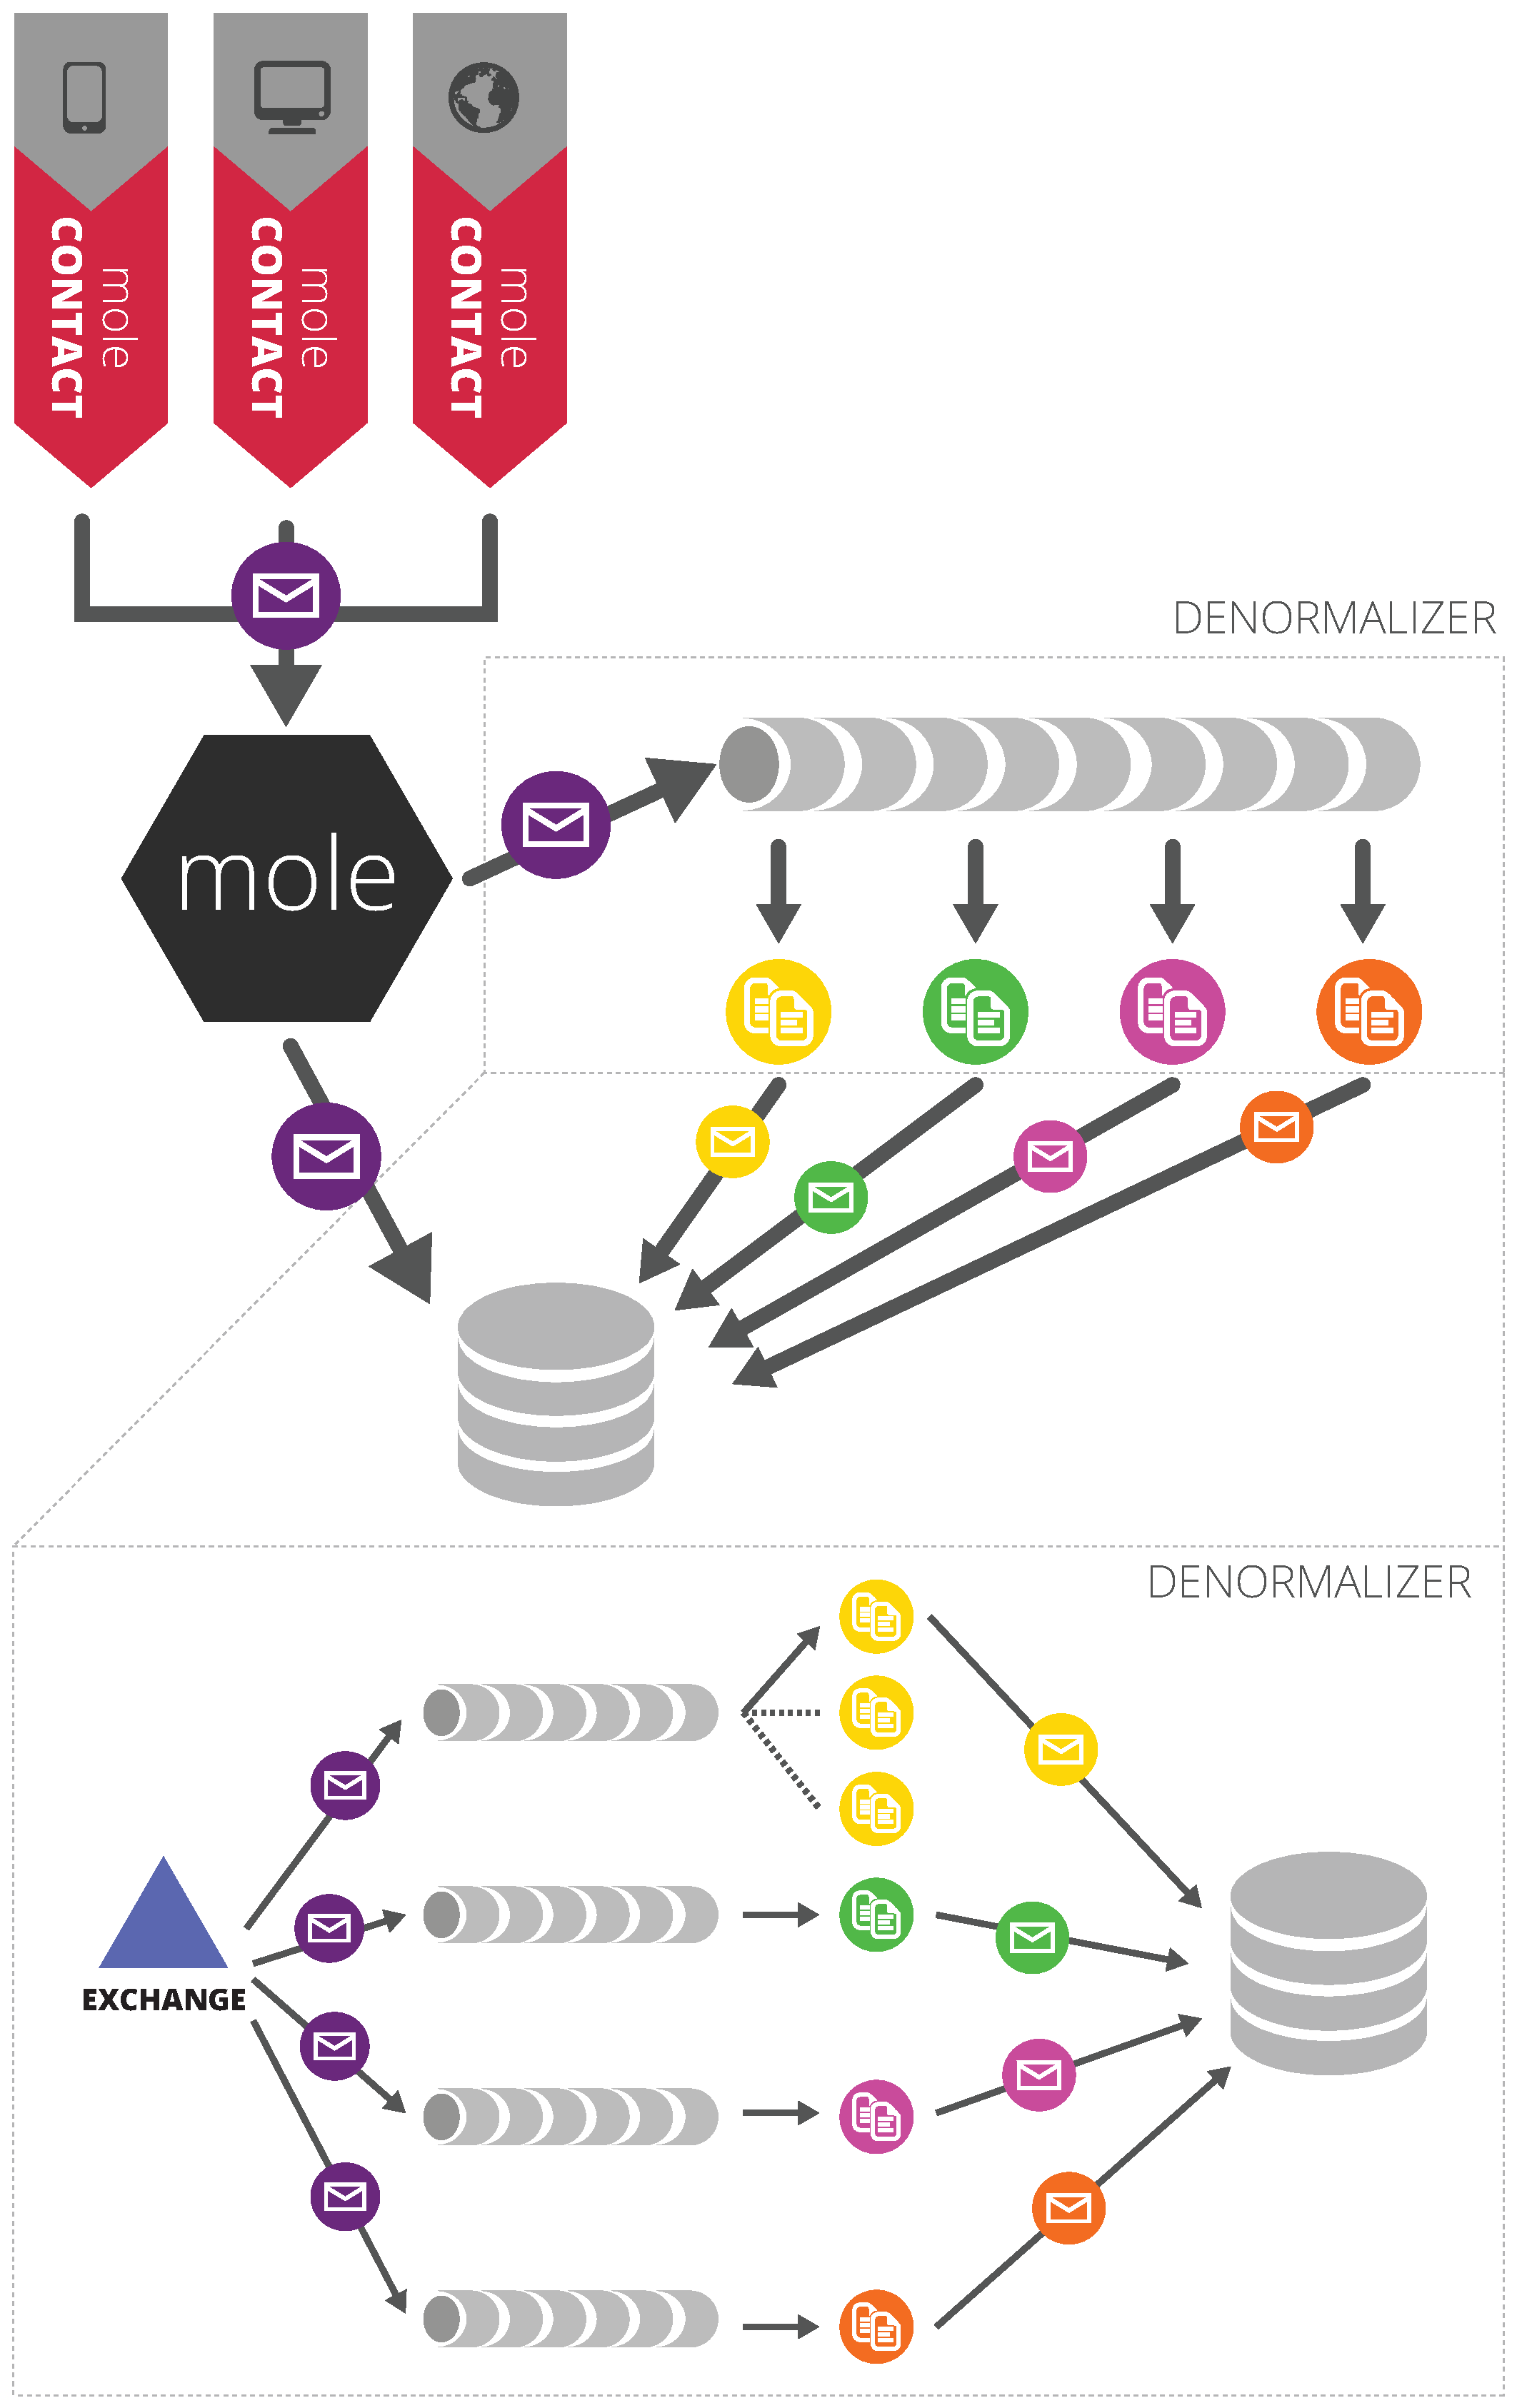
\includegraphics[width=1.0\linewidth]{./img/mole}
\caption[Architettura di mole]{Architettura di mole}
\label{fig:mole}
\end{figure}

In figura \ref{fig:mole} sono mostrate schematicamente la struttura interna del server mole e le comunicazioni instaurate tra i diversi componenti del sistema.
